\documentclass[11pt]{article}
\usepackage{verbatim}
\usepackage{cite}
\usepackage{multirow}
%双栏宏包
\usepackage{flushend,cuted}
%以下两个为数学公式包
\usepackage{amsmath}
\usepackage{amssymb} 
\usepackage[T1]{fontenc}
%图像相关
\usepackage{float}
\usepackage{graphicx}%插入图像
\usepackage{subfigure}%子图
%插入程序代码
\usepackage{listings}
\lstset{language=Matlab}%代码语言使用的是matlab
\lstset{breaklines}%自动将长的代码行换行排版
\lstset{extendedchars=false}%解决代码跨页时,章节标题,页眉等汉字不显示的问题
\textwidth 13.5cm

\author{Liu Zexiang \ \ Fu Mingjian \ \ Gao Yichang}
\title{\textbf{Project Report \\[2ex] A nonlinear programming approach for the college investment problem}}
\date{}
\begin{document}
\maketitle  %生成标题


\section{Introduction}
\paragraph{} This article aims at developing the model of the optimal investment strategy for the Goodgrant Foundation. The strategy will explicitly show the donated schools and their corresponding investment amount.This strategy results from the maximum "ROI" (return on that investment), which is an expectation for the positive effect on the student performance caused by the investment. It is obvious that this parameter is associated with not only the income improvement of the schools and their graduates benefited from the investment, but also the social welfare. For example, the colleges should ensure the bottom amount for the minority students to promote racial equality. Another example is that the donation for the students from low income families should be keep to certain percentage because the investment can narrow the gap between the rich and poor. However, this kind of value cannot be indicated in any financial increase.
\paragraph{} According to the background, we hope to find the optimal strategy according to the following conditions.
\\ 	1. Maximize the return of the investment.
\\ 	2. Ensure the interests of some certain groups.
\paragraph{} Therefore, our team solves the problem in the following steps.
\\ 	1. Evaluate the effects of the variables in IPEDS data to the return of the investment.
\\  2. Construct the function of the total return for each school of the investment.
\\  3. Find the constraints of the investment amount considering students from certain social groups.
\\  4. Find the optimum solution of the function combining the  constraints.
\section{Assumptions}
\paragraph{} 1. The investment only aims at the undergraduates.
\paragraph{} 2. The basic situation of these schools can be almost reflect from the provided data and, generally, the situation will not change.
\paragraph{} 3. The donation is only provided to the colleges whose scorecard data required is complete. 

\section{The Simplified Model}
\subsection{The yield of investment}  
\paragraph{} In order to find the optimal strategy, we compare the profit for each schools acquiring the donation. As the value qualifying the profit, a parameter is defined as $y$ (The yield of investment), which is a ratio of the average income of all the graduates and the roughly educational cost defined as $c$ of them at schools.This value is different for different schools to be the coefficient of the investment for each schools in the return function.
\paragraph{} We choose the "md\_earn\_wne\_p10" (Median earnings of students working and not enrolled 10 years after entry)defined as $p$ to be the standard of the average income of each students and the summation of "IPEDS"(Average net price for Title IV institutions (public institutions), the average annual total family cost of attendance) defined as $c_f$ and "GRAD\_DEBT\_MDN\_SUPP" (Median debt of completers) defined as $d$ to be the cost to provide education to each students in the college.

\begin{align}
y=\frac{p}{c}\\
c=c_f+d
\end{align}

\paragraph{} $y$ for all the potential candidate schools can be written as a vector $Y=(y_1, y_2, y_3, ..., y_N)$. Similarly, the investment for each schools can also be written as $X=(x_1, x_2, x_3, ..., x_N)$.

\subsection{The risk of investment}
\paragraph{} The investment is assumed to be the same amount of scholarship for every students in the school. However, some of the students cannot graduate from  the school for some reasons, the investment for whom is treated as being wasted. So the investment has its own risk. The risk can be reflected by the completion rate vector $R=(r_1, r_2, r_3, ..., r_N)$ which is "C150\_4\_POOLED\_SUPP" (150\% completion rate for four-year institutions, pooled in two-year rolling averages and suppressed for small n size.  For four year school, students are considered to have graduated "on time" if they graduate within 6 years.) or "C200\_L4\_POOLED\_SUPP" (200\% completion rate for less-than-four-year institutions, pooled in two-year rolling averages and suppressed for small n size.  For two year schools, students are considered to have graduated "on time" if they graduate within 4 years.). Therefore, the final $ROI$ function can be defined as:

\begin{align}
ROI=Y^T\*R^T\*X
\end{align}

\subsection{Preferential policies for some social groups}  
\paragraph{} Some constraints should also be developed such as the bottom line of the amount of donation for the minority students. We make a vector $M=(m_1, m_2, m_3, ..., m_N)$ whose elements is the minority students' rate of each potential candidate schools. The vector $N=(n_1, n_2, n_3, ..., n_N)$ indicates the number of students in each schools. So the constraint can be expressed as:
 
\begin{align}
M^T\*N^T\*X\geq\lambda_M\*\frac{M^T\*N}{I^T\*N}
\end{align}

\subparagraph{} ($\lambda_M$ is a coefficient to reflect the extent of the minority preferential treatment. $I$ is N dimensional unit vector.)
 
\paragraph{} The investment should also be distributed to all kinds of majors as fair as possible. We can find the data of percentage of degrees awarded in every schools ("PCIP01" to "PCIP54"). In the similar way, we divided the 54 majors of all the schools into Art, Science and Engineering, and define three vectors $A=(a_1, a_2, a_3, ..., a_N)$ for the percentage of Art degrees awarded in each schools. $S=(s_1, s_2, s_3, ..., s_N)$ for Science and $E=(e_1, e_2, e_3, ..., e_N)$ for Engineering. So the  major constraints can be expressed as:

\begin{align}
A^T\*N^T\*X\geq\lambda_A\*\frac{A^T\*N}{I^T\*N}\\
S^T\*N^T\*X\geq\lambda_S\*\frac{S^T\*N}{I^T\*N}\\
E^T\*N^T\*X\geq\lambda_E\*\frac{E^T\*N}{I^T\*N}\\
\end{align}

\subparagraph{} ($\lambda_A$, $\lambda_S$, $\lambda_E$ are coefficients to reflect the extent of the major being supported. $I$ is N dimensional unit vector.)
\paragraph{} With these constraints, we can find the solution $X$ for maximize the value of ROI function. The solution reflects the exact value of investment for each schools. 

\section{The advanced model} 
\paragraph{} In order to make the model more practical, we improve the design of the ROI function. In reality, the student performance will not be improved in a valid speed. Too little money may not be able to make any changes, but the proper amount of money for the student to keep in a best state of living and learning can develop his potential very well. Too much money can not even make better effect to the student.
\paragraph{} Therefore, we redesign the ROI function of each students profit rate of investment as an "S" curve. When the student get too little money, the performance change mildly. When getting proper amount of money, the student improve his performance swiftly. When he is over-donated, his performance change less and less and finally to his potential limit.
\paragraph{} We can get    

\begin{figure}[H]
\centering
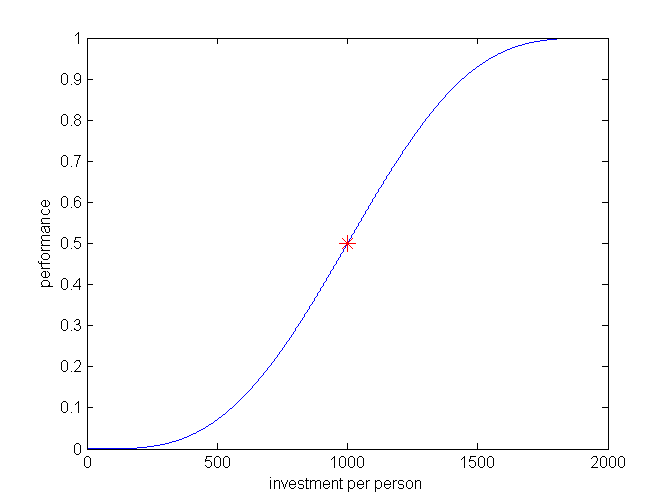
\includegraphics[width=0.5\textwidth]{sfun.png}
\caption{1213123}
\label{arch}
\end{figure}

\end{document}